\section{Workflow}
This section describes the standard workflow for running the \codeName{DCIP2D} inversion. It is provided in a form of a checklist, where elements are linked to other sections of this manual with a more detailed explanation of the concepts. Figure \ref{fig:workflow} shows the workflow guiding the user through the steps of correctly performed inversion. Inverting data is not a one-step process and each inversion should be carried out with an understanding of each step of the process.
%
\begin{figure}[hb]
\centering
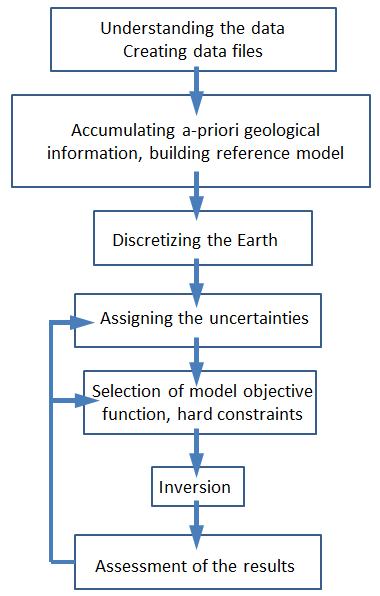
\includegraphics[width=0.4\columnwidth]{workflow}
\caption{Inversion workflow chart.}
\label{fig:workflow}
\end{figure}

\subsection{Understanding the data}
Before inverting the data, please ensure that you have good general understanding of the resistivity/IP data. The following is the checklist of the questions the user should have answers for, prior to preparation of the data for the inversion:
%
\begin{itemize}
\item What is the array configuration?
\item What are the electrode locations and spacing?
\item What are the units of the data?
\item Are the data normalized to unit current?
\item What is the total length of the survey line?
\item Are estimates of the noise on the data available?
\end{itemize}
%
The inversion code assumes that the data are measured voltages due to a unit current in the transmitter. The formats are described in \fileName{Observations} file section. For display purposes however, the \codeName{DCIP2D\_data\_viewer} GUI provided with \prog~will plot data as apparent resistivities.

\subsection{Accumulating prior information; building a reference model}

Prior information includes field geology, drill data, borehole measurements and also an ``educated guess'' about the physical property values and anticipated structures for a particular survey. The goal is to include as much of this information as possible into the final inversion and version ~\version has much flexibility to do this. To be useful, all prior information needs to be connected directly with the physical property in question. Some examples of information that can be included are:
%
\begin{itemize}
\item A listing of the different rock units and the expected range of physical property values.
\item A characteristic geologic model for the deposit (example: typical porphyry geometry).
\item Physical property reference model. The reference model can be defined by a single value or it can be more complicated. Prior knowledge of geology and/or anomaly structure, and associated physical property values, should be incorporated into the reference model.
\item In addition to the reference model it is important to have a sense of its validity. If portions of the reference model arose from point measurements (surface or borehole) then high confidence might exist close to the measurement locations but uncertainty likely increases away from there. If the reference model has a contact zone, then knowledge about the uncertainty in its location is also sought. Thus, in the end, the goal is to have a reference model and also as much knowledge as possible about the data support that generated that model, what is known and what interpolation or hypothesis.
\end{itemize}
%
The above information can be input into the inversion in various ways. The combination of reference models, choice of objective functions to make structures more blocky or smooth, localized weightings for each term in the model objective function, bound constraints on the physical properties, and the use of active and inactive cells allows the user much flexibility to obtain a solution that is compatible with the data and his knowledge about the deposit. This will be addressed further for the workflow item concerned with selecting the model objective function and constraints.

\subsection{Discretizing the Earth}
For the 2D models of the Earth it is assumed that there is no variation of the physical property perpendicular to the line of DCIP data. The earth is represented by a cross-section and this 2D earth is discretized using rectangular cells. Maxwell's equations are solved using a finite volume approach and the accuracy of the solution depends upon the cell size and the total volume. Smaller cells are needed around current or potential electrode sites where the fields or sensitivities change rapidly. The data define a primary region of investigation but the earth model must extend sufficiently far beyond that so the assumed boundary conditions are satisfied (see Figure \ref{fig:fwdMsh} for details). It is essential to verify the modeling mesh via forward modeling prior to inverting the data. A half-space conductivity is forward modeled and the predicted data from this forward modeling can be viewed. The apparent resistivities should not deviate by more than several percent from the half-space values used in the forward simulation.

Topography must be approximated using rectangular cells. When a \fileName{default} mesh is used with UBC-GIF codes, the program builds a discretized 2D Earth. The topography is thus blocky.

\subsection{Assigning uncertainties}
For the inversion, each datum must be assigned an uncertainty. In practice this is challenging because the uncertainty may arise from additive noise, a misplaced electrode, 3D effects that are not modeled by a 2D geometry, numerical modeling errors etc. It is assumed that the error associated with $d_i$, the i$^{th}$ datum, is Gaussian with zero mean and standard deviation $\epsilon$. Estimating values of $\epsilon$ is aided by having some knowledge about the acquisition of data in the field, the equipment used, and the likely sources of noise. A general recipe for assigning uncertainty is:
%
\begin{equation}
\epsilon_i = p*|d_i| + f
\end{equation}
%
where $p$ is a fractional percent and $f$ is a floor in the same units of $d$. The percentage is important when there is large dynamic range in the data. For example, it helps capture errors that arise from electrode mis-allocations. Percentages of 5-7\% are usually reasonable numbers to apply. The floor is a base measurement and reflects the minimum value of the signal that can be measured with the instrument. For example, a percentage (say 20\%) of the average value of the voltages measured with at the largest electrode spacing might suffice as a floor value. It is extremely important not to set the floor to a value that is unrealistically small. If this is done then the inversion algorithm will concentrate its efforts on fitting data that have very small amplitude. An example of using a floor based upon data from a largest electrode separation and a percentage is shown in Figure \ref{fig:DCVscreen}.
%
\begin{figure}[hb]
\centering
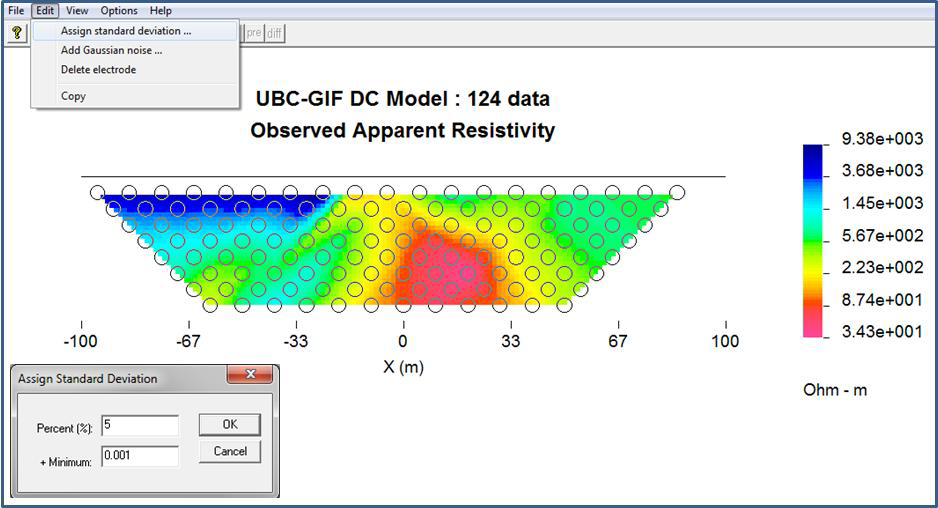
\includegraphics[width=0.5\columnwidth]{assignError}
\caption{Assigning standard deviations using the \codeName{DCIP2D-DATA-VIEWER} GUI.}
\label{fig:DCVscreen}
\end{figure}
%
In Figure \ref{fig:DCVscreen}, the floor value of 0.001 has been assigned followed by 5\% noise in the data. These values can be revised upon the assessment of the inversion results. Errors can also be adjusted for individual data points if you suspect any datum is particularly noisy. For example, it is not uncommon for all data values recorded at one electrode location to have additional noise, due for example to a poor electrical contact, a nearby metallic fence, or other reasons. In standard form, the data misfit $\Psi_d$ is calculated according to equation \ref{eq:phid}. This is appropriate when the data errors are independent and Gaussian with zero mean and standard deviation $\epsilon$. In reality, however, some data might have very large errors. These are \fileName{outliers} and if an incorrect uncertainty is supplied, the weighted difference will be very large and this datum will contribute disproportionately compared to other data. This arises because of the squaring operation in equation \ref{eq:phid}. In order to handle situations where there are outliers, a more robust norm such as a Huber norm can be implemented (See \fileName{Background Theory} for details) can be implemented. The Huber norm is calculated according to equation \ref{eq:Huber}. It has a user-specified coefficient \codeName{c} and acts like a hybrid between $l_1$ and $l_2$ norms. Essentially normalized misfits with a value less than \codeName{c} are evaluated using $l_2$ and those above are evaluated using $l_1$.

\subsection{Selection of model objective function}
The model objective function is specified in equation \ref{eq:disMOF} and is a critical component of the inversion procedure. It is an important conduit for incorporating geologic information. It controls the \fileName{type} of model that will be generated and also geologic detail. The inversion algorithm will find a model that minimizes this function subject to the constraint that the chosen model can generate predicted data that satisfy the misfit criteria. The model objective function can be subdivided into two components: the smallness ($\bvec{W}_s$ components) and smoothness ($\bvec{W}_x$ and $\bvec{W}_z$ components). The components work hand-in-hand and the model objective function will 
%
\begin{enumerate}
\item try to find a model that is as close as possible to a reference model defined either as a half space (by default a half space with a resistivity equal to a weighted average of measured apparent resistivities), or as some other, more complicated model defined by the user (if there is enough prior knowledge), and
\item be as smooth as possible in the X and Z directions. The reference model can be left in or omitted in the derivative terms.
\end{enumerate}

The significance of each component is controlled using the \fileName{alpha} coefficients $\alpha_s, \alpha_x,$ and $\alpha_z,$. Therefore the user can request a model that emphasizes either component 1 (smallness) or component 2 (smoothness). The weighting functions $\bvec{W}_s$, $\bvec{W}_x$ and $\bvec{W}_z$ can be incorporated to enforce more detailed information about the structure. Default values of these coefficients are determined by the program based upon the length scales of the survey and mesh.

Figure \ref{fig:alphaFig} illustrates the effect of changing smallness and smoothness parameters on the inversion results. For the program DCIP2D V5.0, the default specifications for these "alpha" parameters have been found to work well as a first attempt, but experimentation and adjustment of the parameters defining the desired model type may be needed upon assessing the inversion results.
%
\begin{figure}
\centering
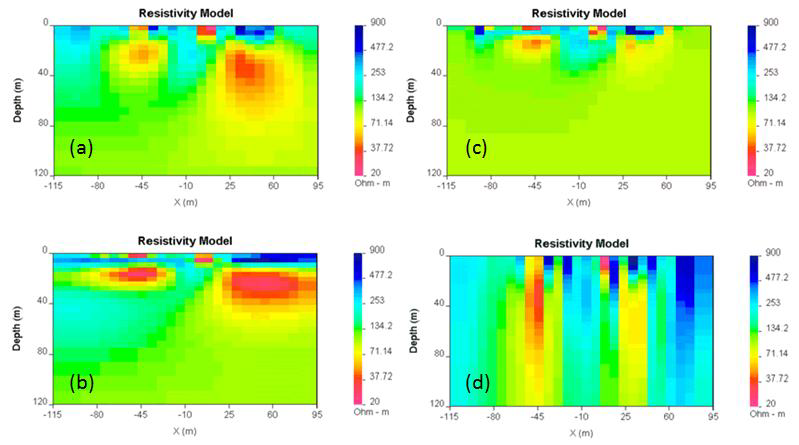
\includegraphics[width=0.5\columnwidth]{alpha}
\caption{Effects of different values of $\alpha_s, \alpha_x, \alpha_z$: (a) [0.01,1,1]; (b) [0.01,1,0.01]; (c) [1,0.01,0.01]; and (d): [0.01,0.01,1]. All models produce the same data.}
\label{fig:alphaFig}
\end{figure}

In addition to the smallness and smoothness coefficients, the new version of \codeName{DCIP2D} offers additional degrees of freedom to edit the model objective function. It is now possible to define the reference model in arbitrary form, as specified in equation \ref{eq:Ekblom}. The parameter $\rho$ which takes values $1\leq\rho\leq2$ controls the character of the model. If $\rho=1$ then the recovered model will tend to be \fileName{blocky} while if $\rho=2$ we obtain our usual $l_2$ smooth model. Again, the reference model can be included, or not, in these terms. Examples of using this new objective function are shown in the \fileName{Examples} section of the manual and additional detail about the numerical implementation is provided in \fileName{Background Theory} section. Bounds constraints can be imposed on the model using the projected gradient method \cite[]{CalamaiMore87}. Each cell can be provided with an upper and lower bound ($m^l$ and $m^u$), such that $m^L_i\le m_i \le m^u_i$.

\subsection{Evaluation of the results}
The following steps should be taken on order to properly assess the results of an inversion:
%
\begin{enumerate}
\item Check the \fileName{log} file. This file contains all the information about the input parameters and the inversion progress. Here are some key concepts of checking the log file:
%
\begin{itemize}
\item Did the inversion end with convergence?
\item Have all the correct files been incorporated and inversion parameters properly set?
\item Was the target misfit achieved?
\item How many iterations were performed?
\end{itemize}
%
\item Predicted data should be compared to the observations using the \codeName{DCIP2D-DATA-VIEWER} GUI. The observed data and the predicted data should look nearly identical. To see variations between them, click the \fileName{diff} button in the data viewing window. This changes the second pseudo-section to a \fileName{misfit map}, which shows the differences between the two data sets (Figure \ref{fig:misfit}). The normalized misfit map (normalized by the assigned standard deviation) should look random, with maximum values of some small percentage of the measured data (based upon noise specifications).
%
\begin{figure}
\centering
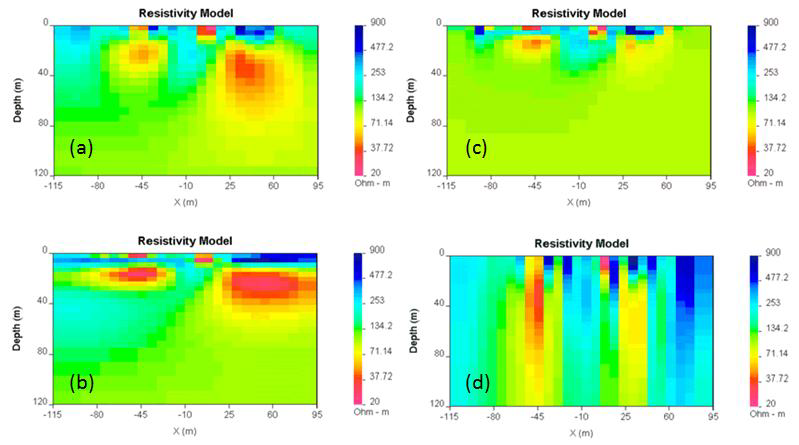
\includegraphics[width=0.5\columnwidth]{alpha}
\caption{(a) Comparison of predicted data with the observed data. (b) Viewing the difference between the predicted data and observed data, normalized by standard deviation.}
\label{fig:misfit}
\end{figure}
%
\item The resulting model should be checked using the \codeName{DCIP2D-MODEL-VIEWER} GUI (provided with \prog) Select \fileName{Padding cells} in the \fileName{Options} menu in this GUI to specify how many padding cells to drop from the display. You can also adjust the minimum / maximum values for the colour scale - necessary for comparing various models (see GUI usage manual for details).
%
The progress of the inversion (or the convergence curve) during its iterations should also be checked (Figure \ref{fig:convGUI}). In the model viewing window, the algorithm's progress can be displayed graphically by selecting the "Curves" toolbar button in the \fileName{View} menu. The resulting graph shows how the values of misfit and model norm varied at each iteration. (\fileName{Model norm} is the value of the model objective function - this is what we are trying to \fileName{minimize}. The algorithm is programmed to add structure gradually in order to find a model that explains the data - i.e. it works on reducing the misfit value (blue curve) until the target misfit is reached. Then it must try to minimize the model norm without changing misfit. Thus, you should see a slight drop in the model norm value (red curve) until no more adjustments can be made to improve the situation.
%
\begin{figure}
\centering
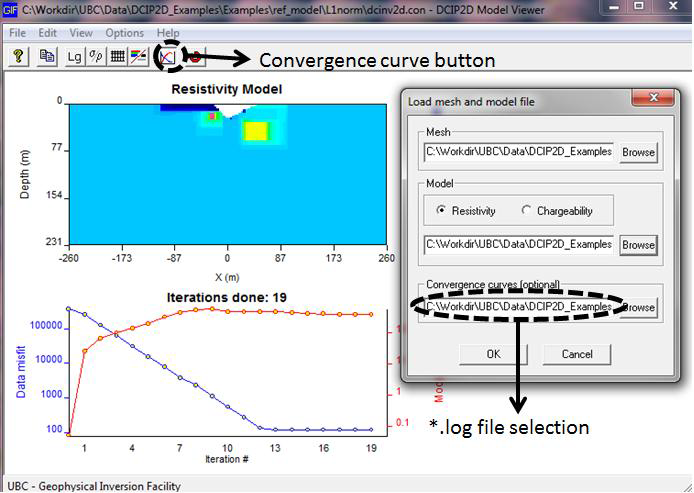
\includegraphics[width=0.5\columnwidth]{convGUI}
\caption{Viewing the model and the inversion progress.}
\label{fig:convGUI}
\end{figure}
%
\item Is the model geologically reasonable? It is important to decide whether the resulting model is geologically reasonable. This final consideration is more subjective. A simple example is shown here, in Figure \ref{fig:fitFig} in which data produced by calculating data over the \fileName{true} 2D model (Figure \ref{fig:fitFig}a) are inverted twice to produce two inversion results which are both inadequate. Figure \ref{fig:fitFig}b shows the model, which is \fileName{underfit} (a model recovered when the target misfit was too large). The program has stopped looking for details when predictions look only somewhat like observations. The image in Figure \ref{fig:fitFig}c show an \fileName{overfit} model (a model recovered when the program has tried too hard to find details that explain every nuance in the observation and resulted in adding structure, which does not exist). In both cases the \codeName{CHIFACT} should be reviewed. In the \fileName{underfit} case it should be made smaller, in \fileName{overfit} case, bigger..
%
\begin{figure}
\centering
\includegraphics[width=0.5\columnwidth]{underOverfit}
\caption{Viewing the model and the inversion progress.}
\label{fig:fitFig}
\end{figure}
%
\end{enumerate}

Another important concept to keep in mind during the verification of the inversion results is the depth of investigation concept. Some of the structure observed in the final model is strongly controlled by the data but other structure is controlled by the details of the regularization functional. By performing two inversions with different reference models or by computing the sensitivities it is possible to obtain some insight regarding which areas of the model are not controlled by the data. These should be removed (or blurred out) from the image before final presentation. An example of this concept is shown in Figure \ref{fig:DOI}. The models in (a) and (b) were respectively recovered from inversions using reference models of a 1000 ohm-m and a 106 ohm-m (given by a default inversion). The DOI analysis was carried out and a threshold value of 0.5 was used to omit parts of the model domain on the model recovered from a 1000 ohm-m background. See figure 14 (c). It is important to note that the model GUI will also perform this analysis given the \fileName{sensitivity.txt} file or multiple output \fileName{model} files. 
%
\begin{figure}
\centering
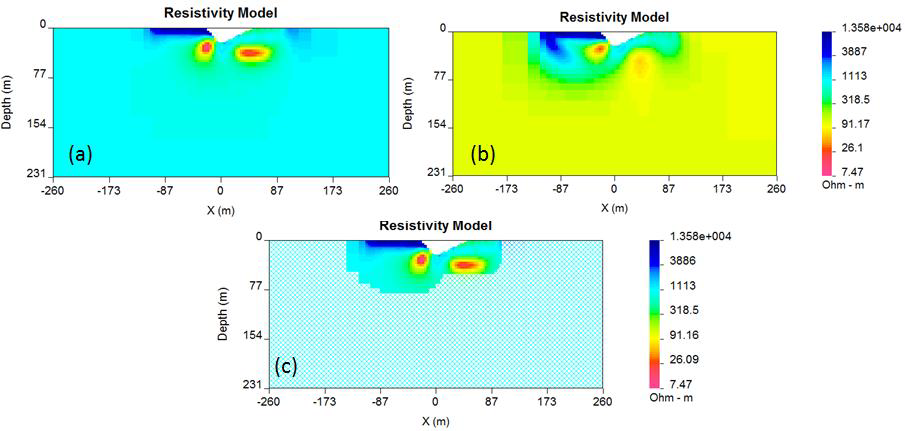
\includegraphics[width=0.5\columnwidth]{doi}
\caption{(a) The model recovered using a 1000 ohm-m background. (b) The model recovered from using a background of 106 ohm-m. (c) The model in (a) truncated to the depth of investigation using a cutoff value 0.5.}
\label{fig:DOI}
\end{figure}
%